\documentclass[a4paper,12pt]{article} 
\usepackage[T2A]{fontenc}			
\usepackage[utf8]{inputenc}			
\usepackage[english,russian]{babel}
\usepackage{float}
\usepackage{amsmath,amsfonts,amssymb,amsthm,mathrsfs,mathtools} 
\usepackage{cancel}
\usepackage{multirow}
\usepackage[colorlinks, linkcolor = blue]{hyperref}
\usepackage{upgreek}\usepackage[left=2cm,right=2cm,top=2cm,bottom=3cm,bindingoffset=0cm]{geometry}
\usepackage{tikz}
\usepackage{graphicx}
\usepackage{subfig}
\usepackage{titletoc}
\usepackage{pgfplots}
\usepackage{xcolor}
\usepackage{wrapfig}
\usepackage{pgfplots}
\pgfplotsset{width=10cm,compat=1.9}

\begin{document}

\begin{titlepage}
		\vspace*{\fill}
		
		\begin{center}
			
\includegraphics[scale=0.8]{MIPT.pdf}
			\\[0.7cm]\Huge Московский Физико-Технический Институт
			\\[2cm]\LARGE Отчет по эксперименту
			\\[0.5cm]\noindent\rule{\textwidth}{1pt}
			\\\Huge\textbf{Определение константы диссоцаиции уксусной кислоты методом кондуктометрии}
			\\[-0.5cm]\noindent\rule{\textwidth}{1pt}
		\end{center}
		
		\vspace*{\fill}
		
		\begin{flushleft}
			Выполняли: \hspace{\fill} Группа:
			\\Розраенко Кирилл и Владимир Лим \hspace{\fill} Б04-202
		\end{flushleft}
	\end{titlepage}

	\setcounter{page}{2}
\section*{Цель работы:}
Исследовать электрические свойства раствора уксусной кислоты и определить его константу диссоциации.
\section*{Оборудование и реактивы:}
Кондуктор "Анион 4100" и измерительная ячейка; раствор KCL с концентрацией 0.01 М; раствор слабого электролита с концецнтрацией 0.01 М (уксусная кислота); стакан стеклянный лабораторный (10 мл); два мерных цилиндра (10 мл); дистилированная вода.
\section*{Теоретическое введение:}

Электрохимия - это раздел физической химии, в котором изучают физико-химические свойства ионных систем, а также процессы и явления на границах раздела фаз с участием заряженных частиц (электронов или ионов)

Электролит - это система, обладающая в жидком или твердом состоянии ионной проводимостью. Соотвественно, различают твердые электролиты, расплавы и растворы электролитов. Электролиты отностятся к проводникам второго рода.

Если раствор электролита поместить в электрическое поле, то ионы начнут смещаться по направлению силовых линий поля. Направленное перемещение ионов электролита будет представлять собой похождение электрического тока через электролит. Чем больше заряд иона и чем большее количество ионов пройдет в секунду через сечение раствора, тем больше будет его электрическая проводимость.

Согласно термодинамической теории, предложенной А.С, Аррениусом, электролит в растворе обладает способностью при растоворении в различных растоворителях распадаться на ионы.

Диссоциация - это химическая реакция между растворителем и электролитом, которая сопровождается выделением или поглощением тепла и изменением объема: $\Delta{H}$ != 0, $\Delta{V}$ != 0. Диссоциация электролитов харакетризуется степенью диссоциации.

Степень диссоциации - это отношение числа молекул электрлита, распавшихся в растворе на ионы, к первоначальному числу молекул.

Константа равновесия реакции диссоциации слабого электролита называется константокй диссоциации.

Электрическая проводимость - это способность растворов электролитов проводить электрический ток.

Молярная электрическая проводимость ($\lambda$) - это электрическая проводимость объема раствора электролита, содержащего 1 моль, растворенного вещества и находящегося между двумя параллельными электродами, расположенными на расстоянии 1 м друг от друга.

Кондуктометрия основана на измерении электриской проводиомсти растворов. На основе электропроводности можно сделать рациональный выбор раствора электролита. Кондуктометрия позволяет автоматизировать контроль производства в процессах, имеющих дело с растворами электролитов или расплавами, определять содержание солей в различных растворах при испарен воды для контроля ее качества.

Степень диссоциации электролита $\alpha_{i}$ рассчитывается по формуле:

\begin{equation} \nonumber
    \alpha_{i} = \frac{\lambda_{i}}{\lambda_{\infty}}
\end{equation}


$\lambda_{i}$ - молярная электрическая проводимость, $\lambda_{\infty}$ - молярная электрическая проводимость при концентрации раствора, стремящейся к нулю.

Константа диссоциации слабого электролита $K_{D}$ определяется для каждого значения концентрации раствора $c_{i}$ по уравнению:

\begin{equation} \nonumber
    K_{D} = \frac{c_i \cdot {\alpha_{i}}^2}{1-\alpha_{i}}
\end{equation}

В итоге получается:
\begin{equation} \nonumber
    K_D = \frac{c_i * {\lambda_i}^2}{\lambda_{\infty}(\lambda_{\infty}-\lambda_i)}
\end{equation}

или:
\begin{equation}
    \frac{1}{\lambda_i} = \frac{1}{\lambda_{\infty}} + \frac{\lambda_i c_i}{K_D {\lambda_{\infty}}^2}
    \nonumber
\end{equation}

Если построить график зависимости $\frac{1}{\lambda} (\lambda c)$, то по тангенсу угла его наклона можно  определить константу диссоциации:

\begin{equation}
    K_D = \frac{1}{\tan({\alpha}){\lambda_{\infty}}^2}
    \nonumber
\end{equation}

\section*{Ход работы:}
Экспериментальная чать данной лабораторной работы состоит из 2-ух эатов:

\begin{enumerate}
    \item Определение нормировочного коэффициента 
    \item Определение константы и степени диссоциации слабого электролита
\end{enumerate}

    \begin{table}[h]
    \centering
    \begin{tabular}{|c|c|c|c|c|c|c|c|c|c|c|}
    \hline
        № & 1 & 2 & 3 & 4 & 5\\ \hline
        $c$, 0.01 моль & 1 & 1/2 & 1/4 & 1/8 & 1/16\\ \hline
        $\chi_{i}$, мкСм/см & 135.1 & 94.0 & 62.9 & 42.7 & 29.0\\ \hline
        $\lambda_{i}$, См*см$^2$/моль & 13.5 & 18.8 & 25.2 & 34.2 & 46.4\\ \hline
        $\alpha_{i} $ & 0.38 & 0.53 & 0.71 & 0.97 & 1.31\\  \hline
    \end{tabular}
    \caption{Результаты измерений}
    \label{table_Delta_nu,tau}
    \end{table}
\paragraph{}

Для $KCL$ получили следующее: $\kappa_{KCl}  = 1,344 * 10^{-3}$ См/см (t = 25°C).

Из специальной таблицы берем удельную электрическую проводимость $\chi_{KCl}$ при 25 °C и 0.01 М. 

Получаем значение: $1,441 * 10^{-3}$ См/см.

Считаем значение нормировочного коэффициента: 

$\varphi$ = $\frac{\chi_{KCl}}{\kappa_{KCl}}$ = 1.072

Молярную электрическую проводимость считаем по следующей формуле: $\lambda_{i} = \frac{1000 \chi_{i}}{ c_i}$

Далее строим график, и по методу наименьших квадратов строим прямую. С тангенса угла наклона находим $K_D$, также при экстрополяции находим значение $\frac{1}{\lambda_{\infty}}$. Получаем следующие значения:

$b = \frac{1}{\lambda_{\infty}}$= 0.028 моль/См $\cdot$ см$^2$;

$\lambda_{\infty}$= 35.7 моль/См $\cdot$ см$^2$;

$k = 65.89 \frac{\text{моль}}{\text{См} \cdot \text{см}^2}^2 \cdot \frac{1}{\text{моль}}$

$K_D = 1.8969 \cdot 10^{-5} $ моль/л. 

\section*{Вывод:}

В ходе работы нам удалось определить константу диссоциации уксусной кислоты методом кондуктометрии. Полученный нами результат с приемлемой точностью совпадает с табличным ($\approx 5 \%$). Для повышения точности при измерениях необходимо использовать растворы с более точной концентрацией. В нашем же случае, в ходе разбавления в 2 раза после каждого измерения, могли возникнуть существенные неточности.

\section*{Приложения:}
\begin{figure}[H]
    \centering
    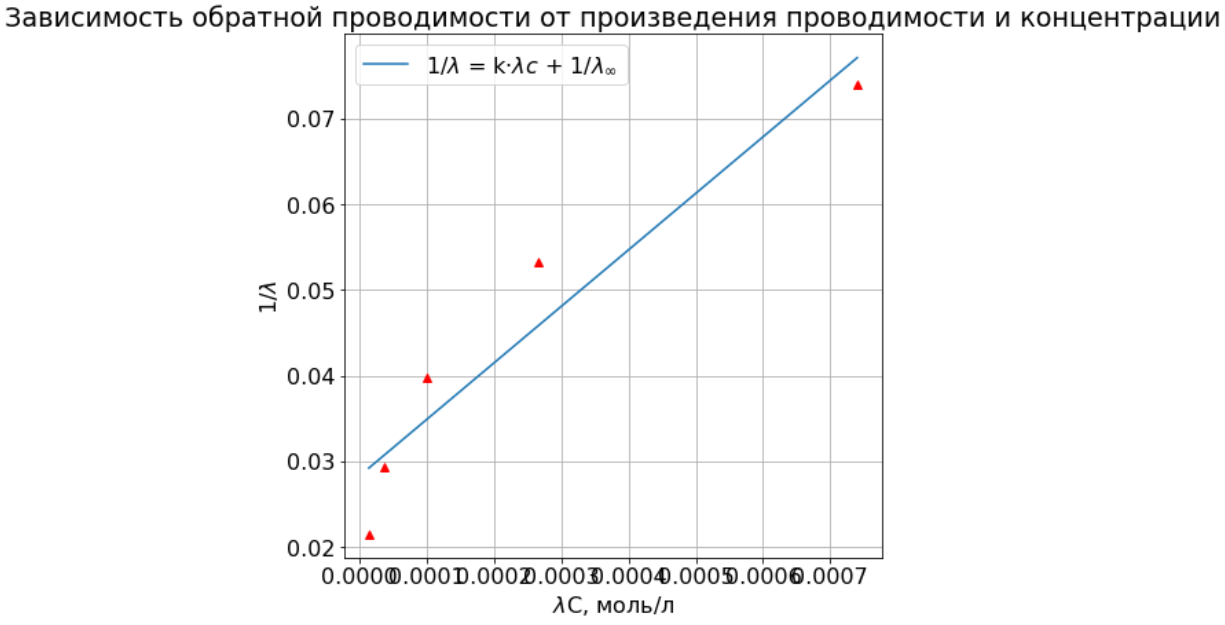
\includegraphics[scale=0.55]{image.png}
    \caption{График $\frac{1}{\lambda}$($\lambda c$)}
\end{figure}
\end{document}

\end{document}
